\documentclass[a4paper,11pt,final]{article}
% Pour une impression recto verso, utilisez plutôt ce documentclass :
%\documentclass[a4paper,11pt,twoside,final]{article}

\usepackage[english,francais]{babel}
\usepackage[utf8]{inputenc}
\usepackage[T1]{fontenc}
\usepackage[pdftex]{graphicx}
\usepackage{setspace}
\usepackage[colorlinks,
            linkcolor=blue,
            anchorcolor=blue,
            urlcolor=blue,
            citecolor=blue
            ]{hyperref}
\usepackage[french]{varioref}
\usepackage{fancyhdr} % 添加页眉页脚
\usepackage{subfigure}
\usepackage{float}
\usepackage{textcomp}
\usepackage{multirow}
\usepackage{array}
\usepackage{longtable}

\newcommand{\reporttitle}{Rapport de Stage \\Année 2013-2014 \vspace{2ex}\\{\large Fouille de Donnée dans la domaine de mobile communication}}

\newcommand{\reportauthor}{Wenyi \textsc{wang}} % Auteur
\newcommand{\reportsubject}{Stage en Entreprise: Stage de fin d'étude} % Sujet
\newcommand{\HRule}{\rule{\linewidth}{0.5mm}}
\setlength{\parskip}{1ex} % Espace entre les paragraphes
%\newcommand{\tabincell}[2]{\begin{tabular}{@{}#1@{}}#2\end{tabular}}%放在导言区%


\hypersetup{
    pdftitle={\reporttitle},%
    pdfauthor={\reportauthor},%
    pdfproducer={\reportauthor},%
    pdfsubject={\reportsubject},%
    pdfkeywords={rapport} {Fouille de donnée} {Mobile Communication} {LTE} {K-MEANS} {Apriori}
}

\pagestyle{fancy}
\lhead{}
\chead{Rapport de Stage}
\rhead{}
\lfoot{}
\cfoot{-\thepage-}
\rfoot{}
\setcounter{page}{3}
\begin{document}
  \pagestyle{empty}
  % Inspiré de http://en.wikibooks.org/wiki/LaTeX/Title_Creation

\begin{titlepage}

\begin{center}

\begin{minipage}[t]{0.48\textwidth}
  \begin{flushleft}
    
\includegraphics [width=30mm]{images/logo-univ.png} \\[0.3cm]
    \begin{spacing}{1.1}
      \textsc{\LARGE Université\\ Jean Monnet \\ \large spécialité Web intelligence}
    \end{spacing}
  \end{flushleft}
\end{minipage}
\begin{minipage}[t]{0.5\textwidth}
  \begin{flushright}
    
\includegraphics [width=30mm]{images/Tsinghua_University_Logo.png} \\[0.5cm]
    \textsc{\LARGE Tsinghuq University\\ \large Department of Electronic Engineering}
  \end{flushright}
\end{minipage}\\ [3.5ex]

\textsc{\Large \reportsubject}\\[0.1ex]
\HRule \\[0.4cm]
{\huge \bfseries \reporttitle}\\[0.2ex]
\HRule \\[10.5ex]

\begin{minipage}[t]{0.3\textwidth}
  \begin{flushleft} \large
    \emph{Auteur :}\\
    \reportauthor
  \end{flushleft}
\end{minipage}
\begin{minipage}[t]{0.6\textwidth}
  \begin{flushright} \large
    \emph{Tuteur de stage en entreprise:} \\
    Vice directeur de labo NGN:\\ yongfeng \textsc{huang} \\
    
    
    \emph{Tuteur de l'université:} \\
        Amaury \textsc{Habrard} \\
  \end{flushright}
\end{minipage}

\vfill
\vfill
{\large De 20 Février 2014 à 20 Juillet 2014}

\end{center}

\end{titlepage}

  \cleardoublepage % Dans le cas du recto verso, ajoute une page blanche si besoin
  %\pagenumbering{roman}
  \tableofcontents % Table des matières
  \thispagestyle{empty}
  \sloppy          % Justification moins stricte : des mots ne dépasseront pas des paragraphes
  \cleardoublepage 
  
  \thispagestyle{empty}
\section*{Remerciements}
\addcontentsline{toc}{section}{Remerciements}

Tout d’abord, je tiens à remercier Amaury Habrard et tous les enseignants de la Spécialité Web Intelligence de l’Université Jean Monnet, aussi les enseignants de Télécom Saint-Etienne et L'école nationale supérieure de Saint-Etienne, qui m’a aidé lors de ces deux années de étude.


Je remercie également M.Yongfeng \textsc{Huang} pour avoir accepter diriger cette stage, il m’a beaucoup conseillé, et les discussions que l’on a pu avoir se sont toujours révélées très intéressantes et instructives.


Je souhaite également adresser mes remerciement à Zheng \textsc{Yang}, Lindong \textsc{Wei} et xian \textsc{wu} ainsi que tout les membres du laboratoire de Next generation Network( \textbf{NGN} ) pour m’avoir soutenu, encouragé et conseillé tout au long de ce stage.


Je tiens à montrer tout ma gratitude envers toutes les personnes qui ont pu m’aider, m’encourager, me soutenir, me remotiver pendant ces années de travail.
  \cleardoublepage
  
  \pagestyle{fancy}  
  \pagenumbering{arabic}
  
%\addcontentsline{toc}{section}{Introduction} % Ajout dans la table des matières
\section{Résumé} 

Pendant ces quatre mois de stage, notre groupe de recherche travaille avec les employés de \textsc{cmcc} ( China Mobile Communications Corporation ) . Le objectif du sujet est: utilise les technique de Fouille de données, étude les données fournir par CMCC, et trouve les relation entre les données et les défaut du système 4G. Nous avons fait plusieurs tentatives pour trouver les résultats, et on a utilise différents logiciel, j'ai utilisé le R, et mon collègue utilise Mathlab, nous avons utilisé plusieurs algorithme (Clusterring, PCA, Association rules, Ajustement). Mais à la fin,  nous avons trouvé que à cause des défaut dans la système d'acquisition, les données ne sont pas correct, et nous ne pouvons pas trouver le résultat comme prévu. Mais les recherches que nous avons fait peut faites-leur savoir comment utilise les technique de fouille de donnée dans la domaine de télécommunication.

\section{Introduction} 
 
Le 3 avril 1973, M. Mation \textsc{cooper} le directeur général de la division communication de Motorola, à effectuer un appel téléphonique à Joel \textsc{engel}, son rival et néanmoins confrère chez \textsf{Belle Labs}. c'est la premier appel téléphonique en extérieur, L'idée du téléphone portable devient une réalité. 

depuis ce jour, le technique développé très rapidement. dans les 20 dernières années, il y a déjà quatre génération des standards pour la téléphonie mobile, non seulement nous pouvons appeler les autres, les nouvelles technologies et les Smart-phones nous permettons aussi envoyer les message, surfer l'Internet, utiliser le service RTSP(Real Timide Streaming Protocol), et le service VoIP (Voice over Internet Protocole),etc.. les services de communication téléphonique sont devenus un outil très important dans notre vie.
 
 \subsection{Introduction du CMCC}
 
Fondé en 3 Septembre 1997, après le regroupement de opérateur des télécommunications en 2008, \textsc{China Mobile Communications Corporation} (\textsf{CMCC})\ref{Fig.sub.1} est devenu un de trois opérateur des télécommunications en Chine (deux autres sont \textsf{China Unicom Co., Ltd.} et \textsf{China Telecom}). Après plusieurs années de développement, il a construit le plus grand réseau de communications mobiles dans le monde, possède la plus grande base d'utilisateurs dans le monde\ref{Fig.sub.2}. En 2013, CMCC a 767 million utilisateurs, 630,2 billion \textyen \qquad de revenu, 121,7 billions \textyen de revenus net, effectif 197,030.
\begin{figure}[H]
	\flushleft
	\subfigure[Logo de China Mobile]{
		\label{Fig.sub.1}
		
\includegraphics[width=1.8in]{images/China_Mobile_2013.png}}\hfill
	\hspace{1in}
%\flushright
	\subfigure[Reseau télécommunication]{
		\label{Fig.sub.2}
		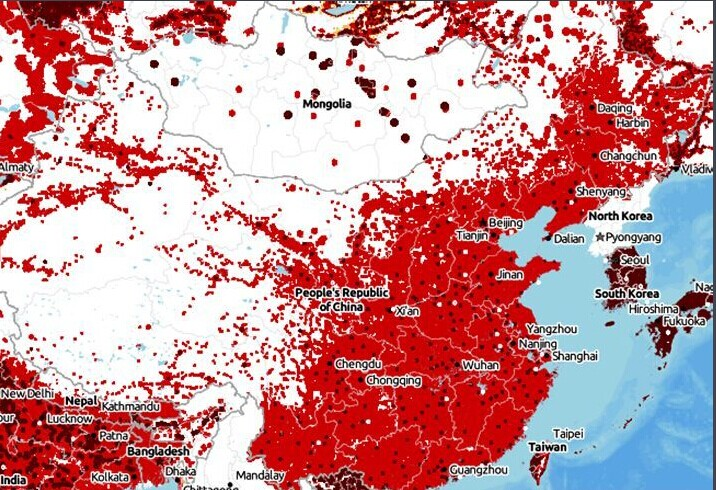
\includegraphics[width=2.0in]{images/reseau.jpg}}
	\caption{CMCC} 
\end{figure}

\subsection{La crise de CMCC}
Mais en même temps, le taux de croissance des nouveaux utilisateur décline de 22,5 \% (2006) à moins de 5\% 2013 \ref{tauxdecroissance}. Et dans la premier 3 mois, l'entreprise une fois considérés comme la plus rentable de Chine, le taux de croissance des revenu net est 0,3\%.

      \begin{figure}[H]
          \centering
          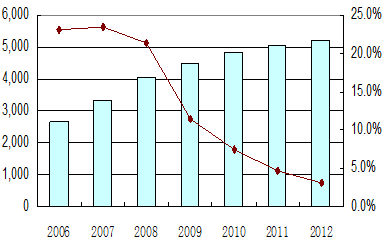
\includegraphics[width=3in]{images/1.png}
          \caption{le taux de croissance est décliner}
          \label{tauxdecroissance}
      \end{figure}
Opérateur des télécommunications Vodafone a fait un étude après il déployé un réseau 3G(\textsf{the third generation of mobile phone mobile communication technology standards}). Comme le réseau 3G permettant des débits (de 2 à 42 Mb/s définis par la dernière génération des réseaux) qui sont bien plus rapides que la génération précédente, par exemple le GSM. Les utilisateur utilisent bien plus souvent le service internet\ref{vodafone1}. Comme ils utilisent plus du service internet, le data ARPU (Average Revenue Per User) augment, mais le voix ARPU décline plus rapide que la montant de data ARPU\ref{vodafone2}. 
 \begin{figure}[H]
 	\flushleft
 	 	\subfigure[Downlink Data Traffic in 2G/3G Network]{
 	 	\label{vodafone1}
 	 	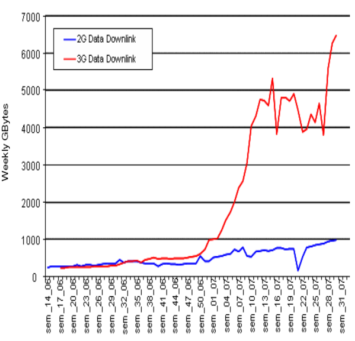
\includegraphics[width=2.0in]{images/4.png}}\hfill
 	\hspace{1in}	 
 	\subfigure[étude de Vodafone]{
 		\label{vodafone2}
 		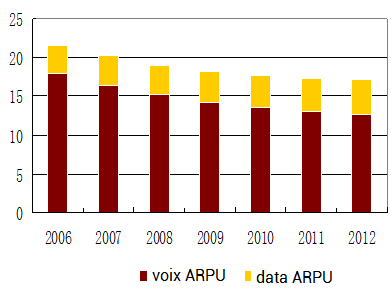
\includegraphics[width=1.8in]{images/2.png}}
 	\caption{Vodafone} 
 \end{figure}
 
Mais l'étude de Orange nous montre que si nous pouvons fournir des nouveaux technologies qui a plus haute débit, les utilisateur utiliseront plus souvent le service data.  \ref{traficparpersonne}
  \begin{figure}[H]
   \centering
   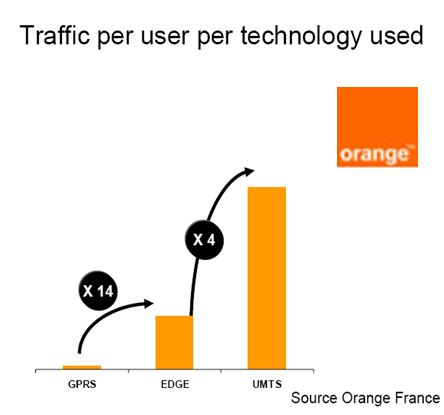
\includegraphics[width=3in]{images/orange.JPG}
   \caption{trafic par personne }
   \label{traficparpersonne}
  \end{figure}
 Des études nous montre nouveaux technologie (comme LTE) peut diminue le prix de revient, qui peut assurer le profit de l'opérateur. Mais déployé les nouveaux matériel coût très cher, en 2009, CMCC dépenser 30 billions \textyen en construit les station pour réseau 3G, et à 2014, CMCC a construit 1,5 million stations, à la fin de cet année, il y aura 1,8 million stations, parmi ces station, il y aura 500 mille stations TD-LTE. En ajoutant des équipement 4G, il peut être mis à niveau un station de 3G à 4G. Donc déployé le réseau 4G n'est pas trop cher, selon l'expérience précédente (de 2G à 3G), les utilisateurs iront utiliser plus le service internet, qui peut assurer le profit de l'entreprise.
      \begin{figure}[H]
          \centering
          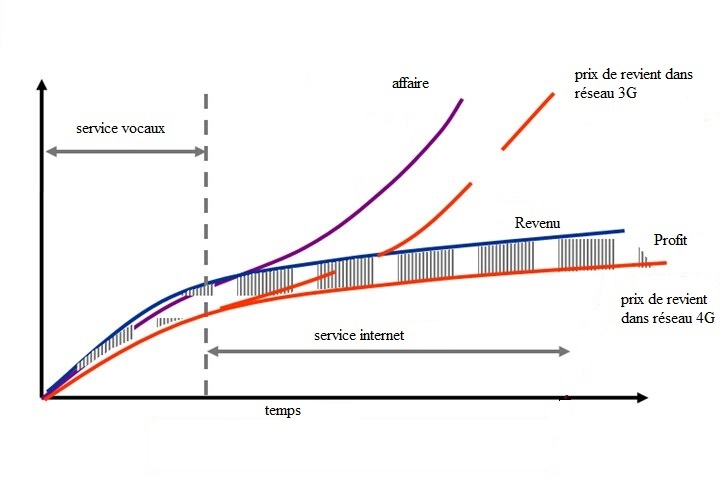
\includegraphics[width=3in]{images/why4G.jpg}
          \caption{4G est plus rentable}
          \label{why4G}
      \end{figure}
  \subsection{L'optimisation du réseau}
A part de la évolution des technologies. Un grand enjeu pour les opérateurs est: l'optimisation du réseau télécommunication. Le réseau de communication mobile est très dynamique, la répartition de la densité du trafic est inégale, fréquence très limité, etc. La configuration du réseau état toujours sous-optimal, et la perception de l'utilisateur n'est pas très bien. Donc tous les opérateurs doivent toujours reconfigurer/optimiser/maintien les paramètre du réseau.
  
Les opérateurs peuvent percevoir les données sur Internet, et utilisent ces informations pour trouver les défauts du système, peut aide l'entreprise optimiser le système.

Mais la optimisation du réseau télécommunication est difficile parce-que: Les technologies d'optimisation de réseau concerné: La technologie de commutation, la technologie sans fil, la configuration et commutation de la fréquence, la signalisation système, l'analyse de trafic, etc. c'est un travail difficile, exiger une meilleure aptitude des employés.  

Actuellement, l'optimisation du réseau dépend principalement à la expérience du personnel. Mais des fois les expériences ne sont pas correct. Par exemple, Si l'entreprise besoin de savoir le congestionné d'un station, il faut envoyer les employé avec des équipement pendant les périodes de pointe, mais on ne sait pas si les résultats sont correct \ref{meseau}.  En outre, souvent un seul type de  donnée ont utilise pour l'analyse et la comparaison pour optimiser les réseau, plutôt que de trouver un solution d'optimisation basées sur toutes les données liées au réseau (telles que les données statistique de trafic, les données d'essai, etc). Et en raison de l'énorme quantité de données, c'est difficile de traite en temps opportun. il est évident que ce méthode est défectueux. Les défauts du système provoque la satisfaction des utilisateurs inférieure, ce qui a conduit à multiplier.
      \begin{figure}[H]
          \centering
          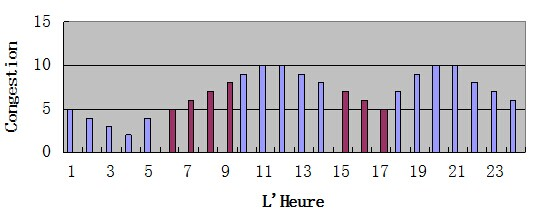
\includegraphics[width=3in]{images/meseau.jpg}
          \caption{Mesure la congestionné d'un station}
          \label{meseau}
      \end{figure}
      
Face à des problèmes complexes, les grands entreprises commence utilise les techniques de Fouille de données. Ce technique peut aide l'entreprise faire les décision plus vite et plus précis.

De ce faire, en Juillet 2013, CMCC a lancé ce projet avec quatre laboratoires dans trois université, ils sont
 \href{http://www.tsinghua.edu.cn/publish/newthuen/index.html}{Tsinghua University}, \href{http://en.sdu.edu.cn/}{Shandong University} et \href{http://www.oice.uestc.edu.cn/en/}{University of Electronic Science and Technology of China}. Le projet inclure trois partiel: Fouille de données, gérés le Clound plateforme et modélisation de l'information dans le système.
 

  \subsection{Introduction du laboratoire}
 De 20 Avril 2014 à 20 Juillet 2014, je fait mon stage chez \href{http://203.91.121.76/joomla/}{laboratoire of Next Generation Network Technology \& Application} \textsf{( NGN )} \ref{Logo NGN}. C'est d'un subordonné de \href{http://www.ee.tsinghua.edu.cn/publish/eeen/3776/index.html}{Research Institute of Network And Human-Machine Speech Comunication}, Département Ingénierie électronique, Tsinghua University. Le laboratoire se trouve dans la ROHM bâtiment.
  \begin{figure}[H]
      \centering
      
\includegraphics[width=3in]{images/NGN.jpg}
      \caption{Logo NGN}
      \label{Logo NGN}
  \end{figure}
Le principaux axes de recherche sont Théorie des réseaux, Architecture de l'Internet, Traitement de l'information Internet, La recherche dans le domaine de la sécurité Internet, Sentiment analyse, Information hiding, etc.

 Mon tuteur professionnel est \href{http://203.91.121.76/joomla/index.php/staff/teacher/83-huangyongfeng}{M. Yongfeng \textsc{huang}}, vice-directeur de la laboratoire NGN. Dans le laboratoire, il y a cinq groupe, chaque groupe a un docteur et son sujet. dans notre groupes, il y a trois personnes, un étudiant de premier année docteur, un étudiant de M1, et une étudiante de Licence troisième année. On utilise R et Rstudio, et Hadoop aussi.
 
 \subsection{Objectif du projet}
Dans cet article, nous avons d'abord présente le réseau communication mobile, ensuite je vais décrire l'état de l'optimisation du réseau. Enfin je présente la mise en place de notre programme de recherche. 
  \cleardoublepage
  
  \section{La première section}


\subsection{Une sous section}

On peut mettre des mots en \emph{italique}, 
en \textsc{petites Majuscules} ou 
en \texttt{largeur fixe (machine à écrire)}.

Voici un deuxième paragraphe avec une formule mathématique simple : $e = mc^2$.

Un troisième avec des \og guillemet français \fg{}.

\subsubsection{Écrire en anglais}

\foreignlanguage{english}{Do you speak French? Does anybody here speak french?}


\subsection{Lites}

\begin{itemize}
\item Liste classique ;
\item un élément ;
\item et un autre élément.
\end{itemize}
\vspace{\parskip} % espace entre paragraphes

\begin{enumerate}
\item Une liste numéroté
\item deux
\item trois
\end{enumerate}
\vspace{\parskip}

\begin{description}
\item[Description] C'est bien pour des définitions.
\item[Deux] Ou pour faire un liste spéciale.
\end{description}
\vspace{\parskip}


\subsection{Références}

Voici une référence à l'image de la figure \ref{bloghiko} page \pageref{bloghiko} et une autre vers la partie \ref{p2} page \pageref{p2}.

On peut citer un livre\,\up{\cite{lpp}} et on précise les détails à la fin du rapport dans la partie références.


\subsection{Note de bas de page}

Voici une note\,\footnote{Texte de bas de page} de bas de page.
Une deuxième\,\footnotemark{} déclarée différemment.
La même note\,\footnotemark[\value{footnote}].

\footnotetext{Il a deux références vers cette note}


\subsection{Figure}

\begin{figure}[!ht]
    \center
    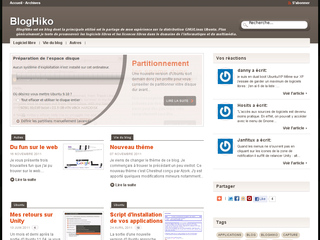
\includegraphics[]{./images/bloghiko.jpg}
    \caption{BlogHiko | taille original}
    \label{bloghiko}
\end{figure}

\begin{figure}[H]
    \center
    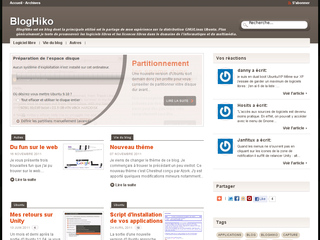
\includegraphics[width=0.5\textwidth]{./images/bloghiko.jpg}
    \caption{BlogHiko | 50\% de la largeur de la page}
\end{figure}



  \cleardoublepage
  
  \section{Citation Wikipédia}
\label{p2}


LaTeX est un langage et un système de composition de documents créé par Leslie Lamport en 198312. Plus exactement, il s'agit d'une collection de macro-commandes destinées à faciliter l'utilisation du \og processeur de texte \fg{} TeX de Donald Knuth. Depuis 1993, il est maintenu par le LaTeX3 Project team. La première version utilisée largement, appelée LaTeX2.09, est sortie en 1984. Une révision majeure, appelée LaTeX2 epsilon est sortie en 1991.

Le nom est l'abréviation de Lamport TeX. On écrit souvent \LaTeX, le logiciel permettant les mises en forme correspondant au logo.

Du fait de sa relative simplicité, il est devenu la méthode privilégiée d'écriture de documents scientifiques employant TeX. Il est particulièrement utilisé dans les domaines techniques et scientifiques pour la production de documents de taille moyenne ou importante (thèse ou livre, par exemple). Néanmoins, il peut aussi être employé pour générer des documents de types variés (par exemple, des lettres, ou des transparents).


  \cleardoublepage
  
  \section*{Conclusion}
\addcontentsline{toc}{section}{Conclusion}

Pendant ce 4 mois de stage, nous avons lu beaucoup de articles, nous avons préparé des dossier et fait des rapport pour le CMCC, aussi nous avons négocié avec les gens du CMCC et les gens du fournisseur de l'équipement. Nous avons perdu beaucoup de temps en négocier et attendre, mais finalement, nous avons trouvé 2 méthode pour résoudre le problème du CMCC.

Dans le rapport, j'ai présenté les algorithmes et la mise en \oe uvre, mais malheureusement, les résultats ne sont pas satisfaisant, nous avons essayé différent paramètre, différente technique, différent logiciel, mais nous n'avons pas trouvé un résultat satisfaisant. Donc nous croyons que cela est causée du fait que la qualité de données est mal. Et parce que nous avons seulement le données erronées, nous ne pouvons pas évaluer notre techniques.

Cependant, pour l'entreprise CMCC, nous avons fait une démonstration en comment utilise les technique de fouille de données avec ses données, et les inconvénients de son système. Et aussi nous montrons que si il a le données non erronées, comme il peut trouver les informations qu'il a besoin.

Pour moi, j'ai utilisé différente algorithme et les logiciel, et j'ai utilisé le langage R pour résoudre les problème. 

J'ai rencontré des bons amis dans le laboratoire, et j'ai acquis des expérience professionnel.

\newpage
\section*{Les travaux futurs}





  \cleardoublepage
  
  \phantomsection\addcontentsline{toc}{section}{Références}
\begin{thebibliography}{ABC}	
    %\bibitem[REF]{reference} auteur. \emph{titre}. édition, année.

    
    \bibitem[1]{specifi}R\&D \textsc{département de }CMCC.   \emph{Interface Specification of China Mobile Signaling Monitoring System(LTE Signal Collection Gateway Part)}.
    \bibitem[2]{kqi}Jianhua DU, Shiwen LU, Fangfeng ZHANG  \emph{Research of KQI Development Methodology in SQM},2008.
    \bibitem[3]{QoE}Luning ZHAO, Zhuo SUN, Wenbo WANG  \emph{Mobile streaming QoE index system and quantify},2012.
    \bibitem[4]{UB} Rui WANG, Fei SU, Zhengdong HAN, Zilong CAI. \emph{The Recessive Problem Mining and Optimization Research of Voice Service Based on User Behaviors}. édition, 2013.
    \bibitem[5]{SC} Lianjiang ZHU, Bingxian MA, Xuequan ZHAO. \emph{Clustering validity analysis based on silhouette coefficient}, 2010.
     \bibitem[6]{AR} Hongyan WANG, Daiwen WU. \emph{Discussion on digging algorithm of correlation rule for numerical attribute}, 2012.
     \bibitem[7]{KmMst}Hao OUYANG, Bo CHEN, Zhenjin HUANG, Meng WANG, Zhiwen WANG. \emph{MST Clustering Algorithme Based on K-Means}. 2014.
\end{thebibliography}

%
\end{document}

